%------------------------------
%
%   FILE: Pop metrics
%   Author: Guillem Ramírez
%   Imoprtant: Graphism to show POP metrics
%
%-----------------------------
\documentclass[crop,tikz]{standalone}
\usepackage[utf8]{inputenc}
\usepackage[T1]{fontenc}

\begin{document}
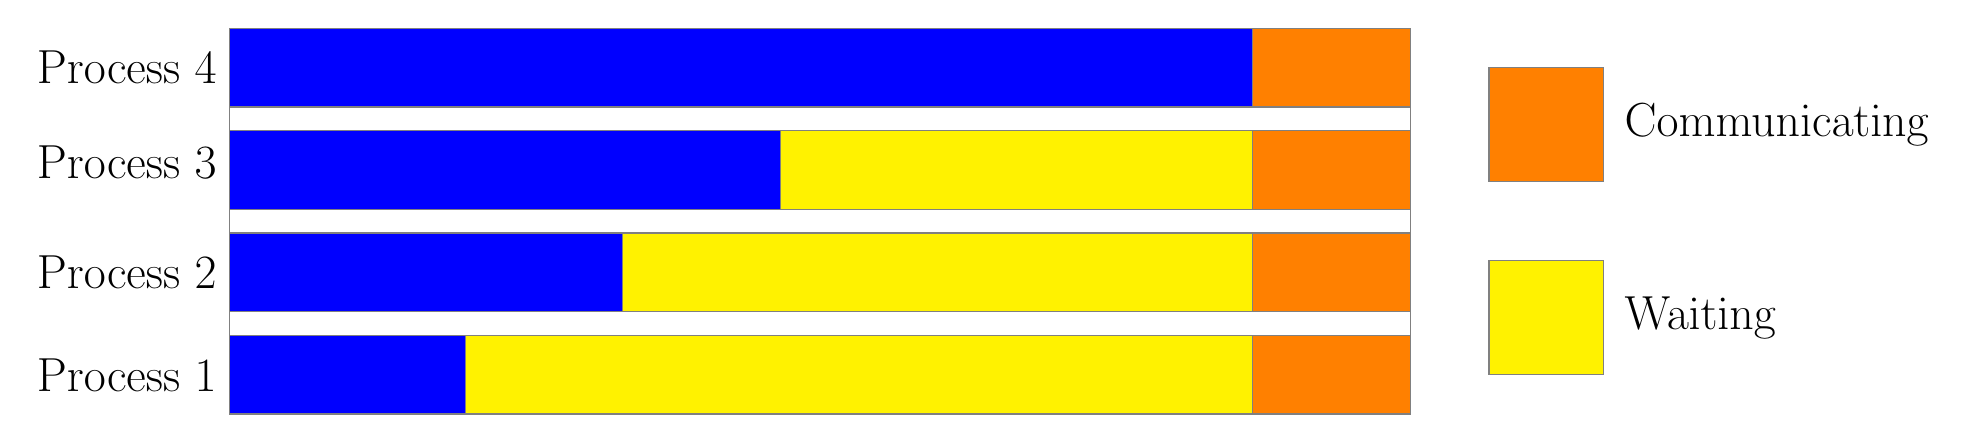
\begin{tikzpicture}
  \filldraw[color=gray, fill=blue] (0,0) rectangle (3,1);
  \filldraw[color=gray, fill=yellow] (3,0) rectangle (13,1);
  \filldraw[color=gray, fill=orange] (13,0) rectangle (15,1);

  \filldraw[color=gray, fill=white] (0,1) rectangle (15, 1.3);
  
  \filldraw[color=gray, fill=blue] (0, 1.3) rectangle (5, 2.3);
  \filldraw[color=gray, fill=yellow] (5, 1.3) rectangle (13, 2.3);
  \filldraw[color=gray, fill=orange] (13, 1.3) rectangle (15, 2.3);

  \filldraw[color=gray, fill=white] (0,2.3) rectangle (15, 2.6);

  \filldraw[color=gray, fill=blue] (0, 2.6) rectangle (7, 3.6);
  \filldraw[color=gray, fill=yellow] (7, 2.6) rectangle (13, 3.6);
  \filldraw[color=gray, fill=orange] (13, 2.6) rectangle (15, 3.6);

  \filldraw[color=gray, fill=white] (0,3.6) rectangle (15, 3.9);

  \filldraw[color=gray, fill=blue] (0, 3.9) rectangle (13, 4.9);
  \filldraw[color=gray, fill=orange] (13, 3.9) rectangle (15, 4.9);

  \node[] at (-1.3, 0.5) {\LARGE{Process 1}};
  \node[] at (-1.3, 1.8) {\LARGE{Process 2}};
  \node[] at (-1.3, 3.2) {\LARGE{Process 3}};
  \node[] at (-1.3, 4.4) {\LARGE{Process 4}};

  \filldraw[color=gray, fill=yellow] (16, 0.5) rectangle (17.45, 1.95);
  \filldraw[color=gray, fill=orange]  (16, 2.95) rectangle (17.45, 4.4);

  \node[anchor=west] at (17.6, 1.225) {\LARGE{Waiting}};
  \node[anchor=west] at (17.6, 3.675) {\LARGE{Communicating}};

%  \node[inner sep=0pt] (flag) at (10.08, 1.1)
%    {\includegraphics[width=0.03\textwidth]{vector-flag.png}};
\end{tikzpicture}
\end{document}
